\documentclass[11pt]{article}\usepackage[]{graphicx}\usepackage[]{color}
%% maxwidth is the original width if it is less than linewidth
%% otherwise use linewidth (to make sure the graphics do not exceed the margin)
\makeatletter
\def\maxwidth{ %
  \ifdim\Gin@nat@width>\linewidth
    \linewidth
  \else
    \Gin@nat@width
  \fi
}
\makeatother
\usepackage{pdfpages} 
\definecolor{fgcolor}{rgb}{0.345, 0.345, 0.345}
\newcommand{\hlnum}[1]{\textcolor[rgb]{0.686,0.059,0.569}{#1}}%
\newcommand{\hlstr}[1]{\textcolor[rgb]{0.192,0.494,0.8}{#1}}%
\newcommand{\hlcom}[1]{\textcolor[rgb]{0.678,0.584,0.686}{\textit{#1}}}%
\newcommand{\hlopt}[1]{\textcolor[rgb]{0,0,0}{#1}}%
\newcommand{\hlstd}[1]{\textcolor[rgb]{0.345,0.345,0.345}{#1}}%
\newcommand{\hlkwa}[1]{\textcolor[rgb]{0.161,0.373,0.58}{\textbf{#1}}}%
\newcommand{\hlkwb}[1]{\textcolor[rgb]{0.69,0.353,0.396}{#1}}%
\newcommand{\hlkwc}[1]{\textcolor[rgb]{0.333,0.667,0.333}{#1}}%
\newcommand{\hlkwd}[1]{\textcolor[rgb]{0.737,0.353,0.396}{\textbf{#1}}}%
\let\hlipl\hlkwb

\usepackage{ulem}

\usepackage{framed}
\makeatletter
\newenvironment{kframe}{%
 \def\at@end@of@kframe{}%
 \ifinner\ifhmode%
  \def\at@end@of@kframe{\end{minipage}}%
  \begin{minipage}{\columnwidth}%
 \fi\fi%
 \def\FrameCommand##1{\hskip\@totalleftmargin \hskip-\fboxsep
 \colorbox{shadecolor}{##1}\hskip-\fboxsep
     % There is no \\@totalrightmargin, so:
     \hskip-\linewidth \hskip-\@totalleftmargin \hskip\columnwidth}%
 \MakeFramed {\advance\hsize-\width
   \@totalleftmargin\z@ \linewidth\hsize
   \@setminipage}}%
 {\par\unskip\endMakeFramed%
 \at@end@of@kframe}
\makeatother

\definecolor{shadecolor}{rgb}{.97, .97, .97}
\definecolor{messagecolor}{rgb}{0, 0, 0}
\definecolor{warningcolor}{rgb}{1, 0, 1}
\definecolor{errorcolor}{rgb}{1, 0, 0}
\newenvironment{knitrout}{}{} % an empty environment to be redefined in TeX

\usepackage{alltt}
\usepackage{graphicx, fancyhdr}
\usepackage{amsmath, amsfonts}
\usepackage{color}
\usepackage{hyperref}

\newcommand{\blue}[1]{{\color{blue} #1}}

\setlength{\topmargin}{-.5 in} 
\setlength{\textheight}{9 in}
\setlength{\textwidth}{6.5 in} 
\setlength{\evensidemargin}{0 in}
\setlength{\oddsidemargin}{0 in} 
\setlength{\parindent}{0 in}
\newcommand{\ben}{\begin{enumerate}}
\newcommand{\een}{\end{enumerate}}


\lhead{STAT 305}
\chead{Solution \#2} 
\rhead{Due Thursday, Sep. $12^{th}$ in the class}
\lfoot{Fall 2019} 
\cfoot{\thepage} 
\rfoot{} 
\renewcommand{\headrulewidth}{0.4pt} 
\renewcommand{\footrulewidth}{0.4pt} 

\def\Exp#1#2{\ensuremath{#1\times 10^{#2}}}
\def\Case#1#2#3#4{\left\{ \begin{tabular}{cc} #1 & #2 \phantom
{\Big|} \\ #3 & #4 \phantom{\Big|} \end{tabular} \right.}
\IfFileExists{upquote.sty}{\usepackage{upquote}}{}
\begin{document}
\pagestyle{fancy} 

Show \textbf{all} of your work on this assignment and answer each question fully in the given context. \\
You will want to understand Exercise 1 from Section 2.1 before attempting the following questions.  
Your answers should be written in complete sentences.
It is possible that a drawing or table may help make your thoughts more concrete or illustrate a concept that would be difficult to describe in words alone - if so I encourage you to use one.\\

\emph{Please} staple your assignment!

\begin{itemize}

\item \textbf{Problem1: Chapter 2, Section 3, Exercise 1 (page 47)[5 pts]} \\
Possible controlled variables are: operator, launch angle, launch force, paper clip size, paper manufacturer, plane constructor, distance measurer and wind.\\
The response is Flight Distance.\\
The experimental variables are Design, Paper Type, and Loading Condition. \\
Concomitant variables might be wind speed and direction( if these cannot be controlled), ambient temperature, humidity and atmospheric pressure. 

\item \textbf{Problem2: Chapter 2, Section 3, Exercise 5 (page 47)[5 pts]}\\
For the delta/ construction/ with clip condition(for example), flying the same plane twice would provide information about flight-to-flight variability for that particular plane. This would be useful if you are only interested in making conclusions about that particular plane. If you are interested in generalizing your conclusions to all delta design planes made with construction paper and loaded with a paper clip, then re-flying the same airplane does not provide much more information. But making and flying two planes for this condition would give you some idea of variability among different planes of this type, and would therefore validate any general conclusions made from the study. This argument would be true for all 8 conditions, and would also apply to comparisons made among the 8 conditions. 

\item \textbf{Problem3: Chapter 2, End of chapter exercise, Exercise 7 (page 65)[10 pts]}\\
(a) Label the widgets $ 1, 2, \cdots, 354$. Select a random sample of size five either through software, random table or even on RANDOM.org. One possible sample is the widgets labeled 121, 91, 134, 313, and 249.\\

(b) Label the 12 experimental runs as follows:
\begin{center}
	\begin{tabular}{|c|c|c|}
		\hline
		Labels & Level of A &  Level of B\\
		\hline
		1, 2 & 1 & 1\\
		3, 4 & 2 & 1\\
		5, 6 & 1 & 2\\
		7, 8 & 2 & 2\\
		9, 10 & 1 & 3\\
		11, 12 & 2 &3\\
		\hline
	\end{tabular}
	
\end{center}
Use the following coding for the test labels:
\begin{center}
	\begin{tabular}{|c|c|}
		\hline
		Table Number & Test Label\\
		\hline
		01-05 & 1\\
		06-10 & 2\\
		11-15 & 3\\
		16-20 & 4\\
		21-25 & 5\\
		26-30 & 6\\
		31-35 & 7\\
		36-40 & 8\\
		41-45 & 9\\
		46-50 & 10\\
		51-55 & 11\\
		56-60 & 12\\
		\hline
	
	\end{tabular}
\end{center}
Now, moving through Table B-1 choosing two digits at a time, ignoring numbers between 61 and 00, and those corresponding t runs that have already been picked. Order runs in the same order that their corresponding 2 digit number are picked from the table. Using this method, an starting from where I left off in part (a), the order would be 3, 2, 11, 7, 6, 1, 4, 9, 12, 5, 8, 10.\\
\textbf{Note:} The whole process of taking the sample can also be done through software or RANDOM.org as was done in part (a).
\item \textbf{Problem4: Chapter 2, End of chapter exercise, Exercise 11 (page 65)[5 pts each part]}\\
(a) Control the extraneous variable heat by using only one bar for the entire study. This will eliminate any heat-to-heat variability.\\
(b) Advantage: may reduce baseline variation (background noise) in the response, making it easier to see any difference between the 2 brands. \\
Disadvantage: One heat may not be representative of all such material that the drills would be used on. 
Controlling makes the expriment more artificial- It will be harder to generalize conclusions from this heat to others.
\item \textbf{Problem5: Chapter 3, Section 2,  Exercise 1 (page 92)[5 pts each part]}\\
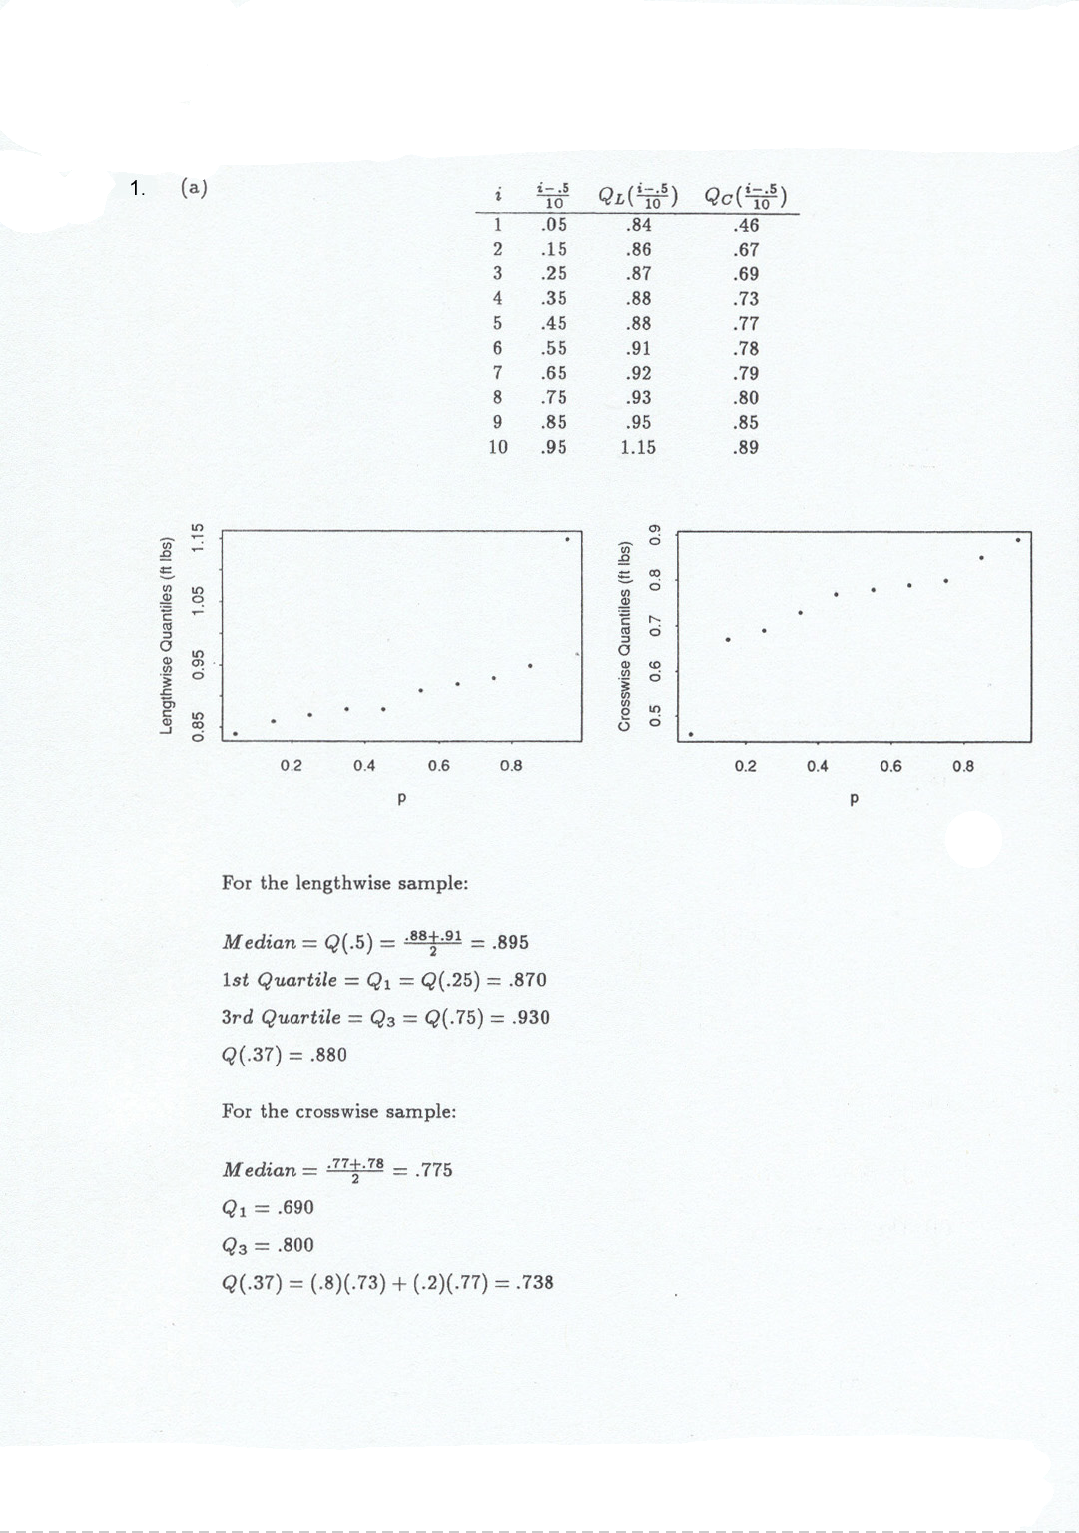
\includepdf[page={1, 2}]{ch3s1}
\item \textbf{Problem6: JMP Assignment. [5 pts each part]} 

   Computing is one of the most important parts of modern data analysis. A large part of data science simply wouldn't exist without the tools developed by scientists working at the intersections of computer science, mathematics, and statistics. 
   Because of that, there will inevitably be parts of this course where a statistical computing tools are needed. SAS and R are the two main languages used by statisticians, though Python, Julia, F\#, C++ and others are also common.
   SAS has a software called JMP ("Jump") that makes doing statistical analyses simpler - it is more powerful than Excel or your calculator but requires little in the sense of coding making the learning curve much lower. 
   We will be using it this semester. There are labs in Snedecor Hall with the software pre-installed, but it is free for students and I encourage you to download a copy for yourself using the link below.

   Download: \href{https://www.stat.iastate.edu/statistical-software}{https://www.stat.iastate.edu/statistical-software}

   In this problem, we will work through the tutorial found at \href{http://web.utk.edu/~cwiek/201Tutorials/}{http://web.utk.edu/$\sim$cwiek/201Tutorials/}. Download and install \texttt{JMP} or find a computer with it already installed. Once you have done this, complete the following sections from the the tutorial linked above. For each part, print and include the table or graph produced. (Note: You can save the plots/tables and combine them in a single document).\\
\textbf{NOTE:} You should use the data set available on the tutorial to finish this exercise, but if you have any data sets of your own, I'd be more than happy to see you use JMP to make some summarizations on your data set. 

   \begin{enumerate}
      \item Creating a JMP data table
      \item Bar Chart
      \item Pie Chart
      \item Mosaic Plot
      \item Histogram and Box Plot
      \item Stem and Leaf Plot
      \item Side-by-Side Box Plots
      \item Calculating Summary Statistics of Quantitative Data
   \end{enumerate}

Total: 90 pts


















\end{itemize}


\end{document}
